\chapter{Results}
% \textit{\ifdraft{In this section you discuss any issues that came up while developing
% the system.  If you found something particularly interesting,
% difficult, or an important learning experience, put it here.  This is
% also a good place to put additional figures and data.}}

\section{Using a robot to create image data set}\label{resrobotcontrol}

\subsection*{Tests}
Robot manipulator performance was measured by making four tests and taking time, iterations and interventions. The performance can been seen in \textit{Table \ref{tab:testonrobot}}.

\begin{table}[h]
\resizebox{\textwidth}{!}{%
\begin{tabular}{clccccccc}
\hline
\textit{Test\#} &
  \textit{Item} &
  \textit{\begin{tabular}[c]{@{}c@{}}Start pos\\ {[}x, y, z{]}\end{tabular}} &
  \textit{Iterations} &
  \textit{\begin{tabular}[c]{@{}c@{}}Operator\\ intervention\end{tabular}} &
  \textit{\begin{tabular}[c]{@{}c@{}}Time \\ {[}sec{]}\end{tabular}} &
  \textit{\begin{tabular}[c]{@{}c@{}}Did it \\ finish?\end{tabular}} &
  \textit{\begin{tabular}[c]{@{}c@{}}Movement \\ time {[}sec{]}\end{tabular}} &
  \textit{\begin{tabular}[c]{@{}c@{}}Intervention\\ vs.  Iterations\end{tabular}} \\ \hline
\multicolumn{1}{c|}{1} &
  \begin{tabular}[c]{@{}l@{}}Nivea \\ Cleansing Milk\end{tabular} &
  \begin{tabular}[c]{@{}c@{}}{[}0.336, \\ 0.045, \\ 0.097{]}\end{tabular} &
  100 &
  2 &
  1277.2 &
  Yes &
  12.77 &
  2\% \\
\multicolumn{1}{c|}{2} &
  \begin{tabular}[c]{@{}l@{}}Alberto \\ Balsam coconut\end{tabular} &
  \begin{tabular}[c]{@{}c@{}}{[}0.343, \\ 0.043, \\ 0.107{]}\end{tabular} &
  100 &
  0 &
  1254.2 &
  Yes &
  12.54 &
  0\% \\
\multicolumn{1}{c|}{3} &
  \begin{tabular}[c]{@{}l@{}}Nivea \\ Cleansing Milk\end{tabular} &
  \begin{tabular}[c]{@{}c@{}}{[}0.340 , \\ 0.044, \\ 0.098{]}\end{tabular} &
  300 &
  6 &
  3799.1 &
  Yes &
  12.66 &
  2\%  \\
\multicolumn{1}{c|}{4} &
  \begin{tabular}[c]{@{}l@{}}Alberto \\ Balsam coconut\end{tabular} &
  \begin{tabular}[c]{@{}c@{}}{[}0.333 , \\ -0.040, \\ 0.118{]}\end{tabular} &
  300 &
  1 &
   3774.4&
  Yes &
   12.58 &
  0.33\% \\ \hline
\multicolumn{7}{r}{\textbf{Average:}} &
  12.64 &
  1.08\% \\ \hline
\end{tabular}%
}
\caption{Test made on the robot and code performance}
\label{tab:testonrobot}
\end{table}
\clearpage
%%%%%%%%%%%%%%%%%%%%%%%%%%%%%%%%%%%%%%%%%%%%%%%%%%%%%%%%%%%%%%%%%%%%%
\section{Automatic labelling}\label{rescamera}
The automatic labelling is not simple, since you need to look at few things such as lighting conditions, light reflection from objects, shades and more. So two methods were tested that were described in the methods chapter. 
\subsection{Before vs. after}
The results from the Before and After method was fine, but in some cases when the bottles area intersect each other it can't find the right bounding box. 
\begin{figure}[ht]
    \centering
    % include first image
    \subfloat[Before]{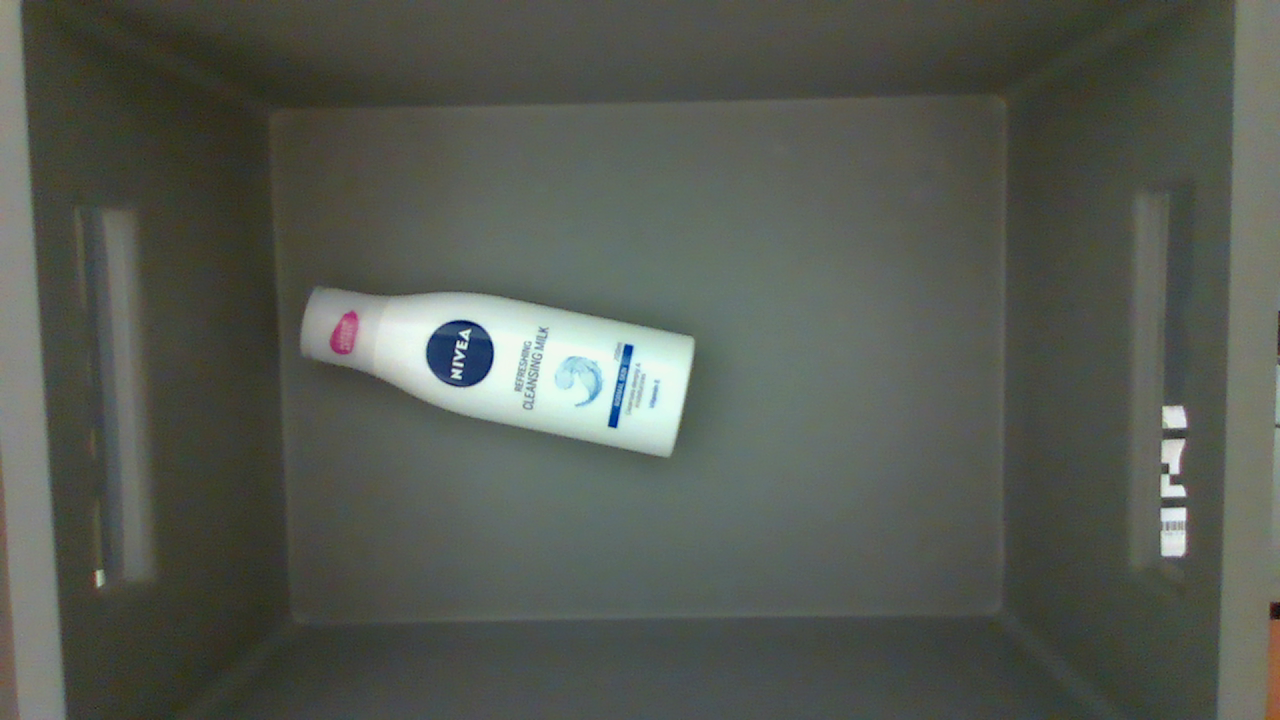
\includegraphics[width=0.495\textwidth]{graphics/9before.png}}
    \hfill
    \subfloat[After]{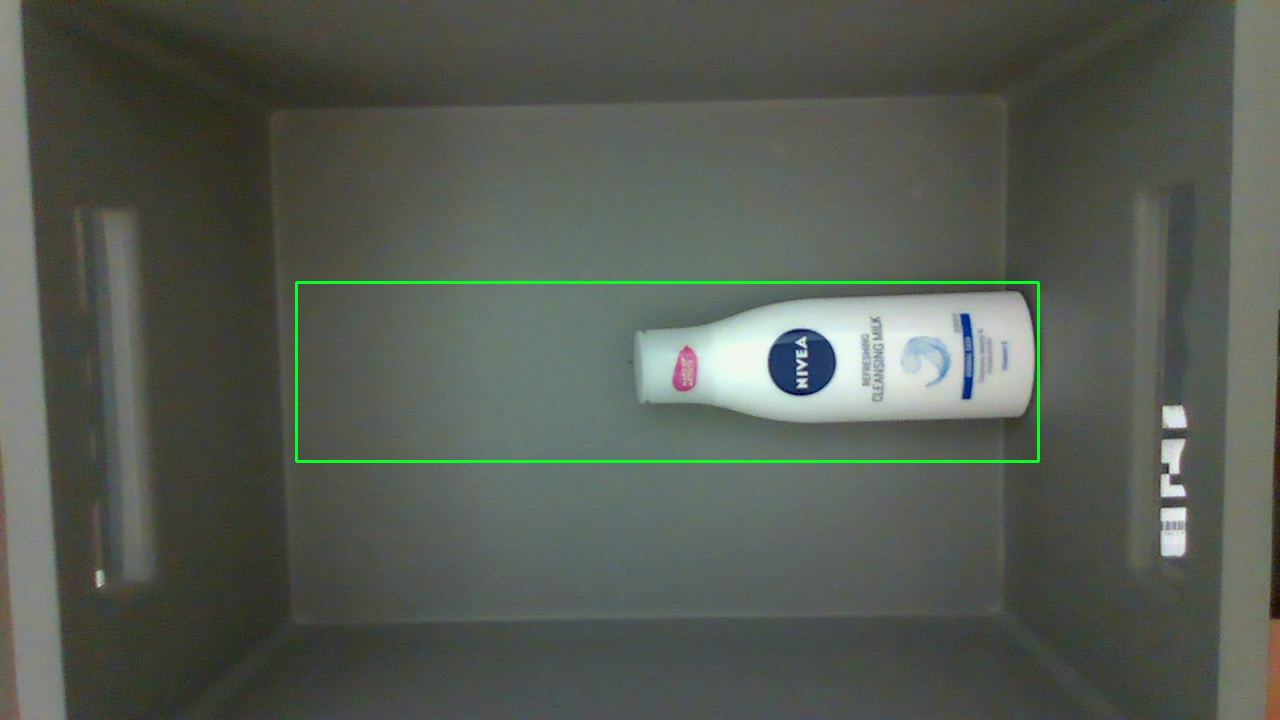
\includegraphics[width=0.495\textwidth]{graphics/9after.png}}
    \hfill
    \subfloat[Contours]{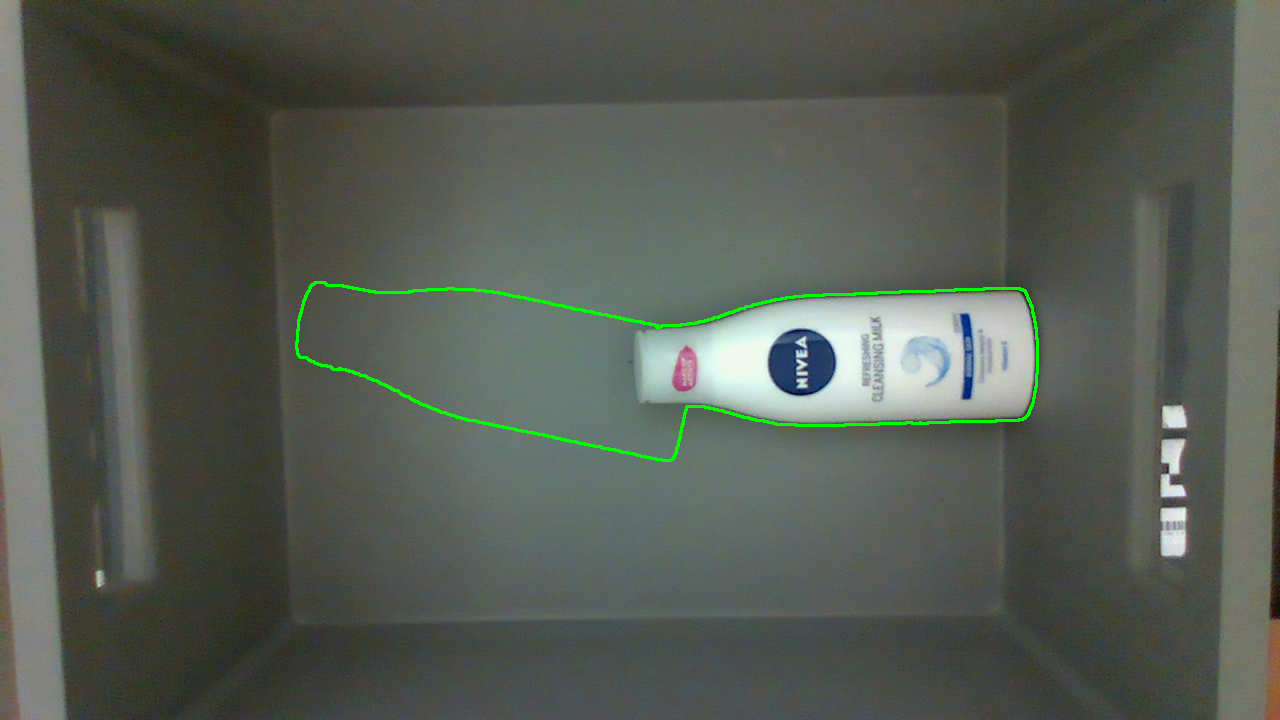
\includegraphics[width=0.495\textwidth]{graphics/9filled.png}}
    \hfill
    \subfloat[Masked]{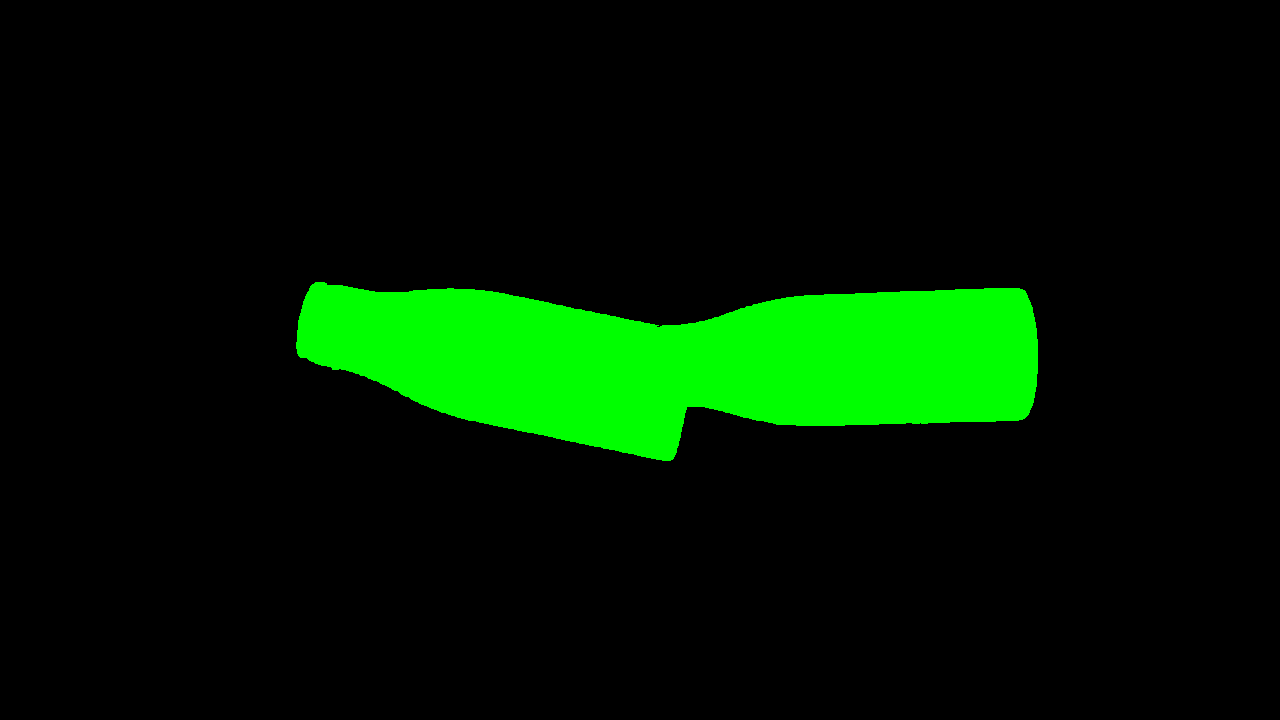
\includegraphics[width=0.495\textwidth]{graphics/9masked.png}}
    \caption{Image Difference with OpenCV and Python}
    \label{figure: imagework}
\end{figure}

As can been seen in the \textit{Figure \ref{figure: imagework}} this would not work so another method would be needed to find the right bounding box automatically. In the figure the before, after, contoured difference and masked contour can be seen. 

\subsection{Empty bin vs. Object in the bin}
The second method showed an increase in performance and almost perfect results, since it needed to go through two functions of object finding. So it would work for dark items, light items or strange shaped items.

As can been seen in the \textit{Figure \ref{figure: labelling}} this method works to create a automatic labelled data.

\begin{figure}[h]
    \centering
    % include first image
    \subfloat[Alberto Balsam]{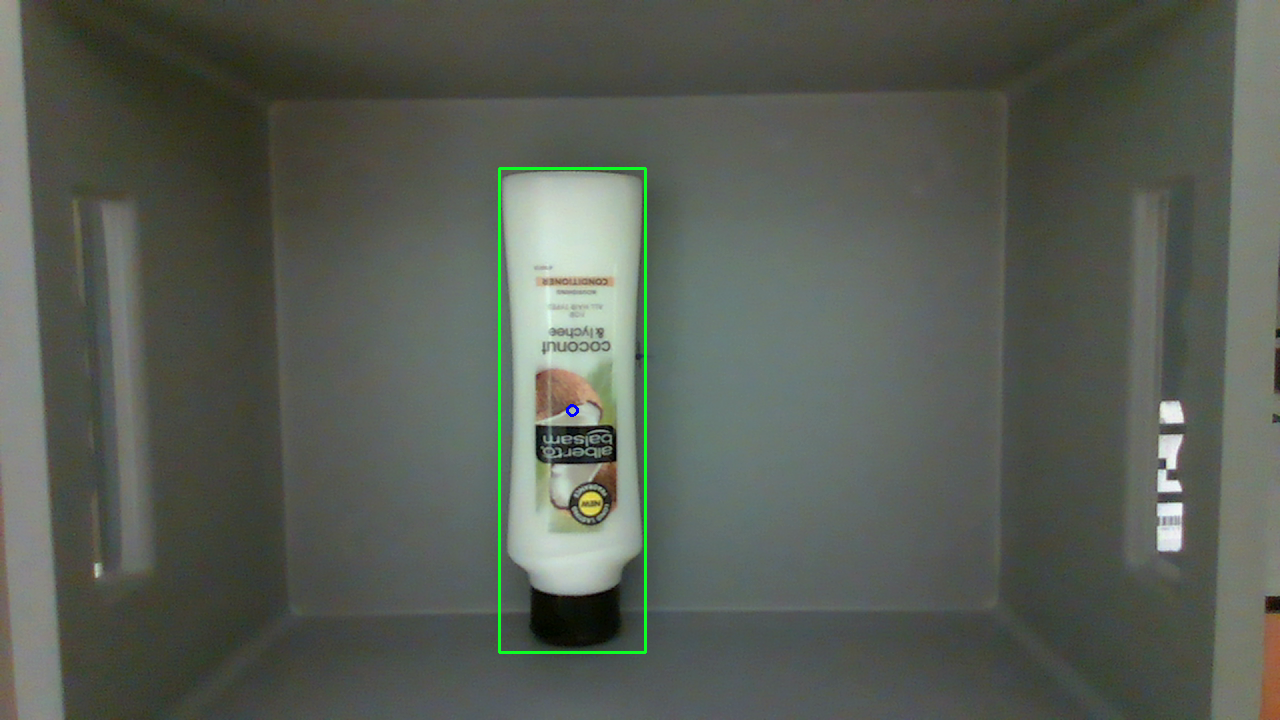
\includegraphics[width=0.495\textwidth]{graphics/results/albertobalsam100_51.png}}
    \hfill
    \subfloat[Nivea Cleansing Milk]{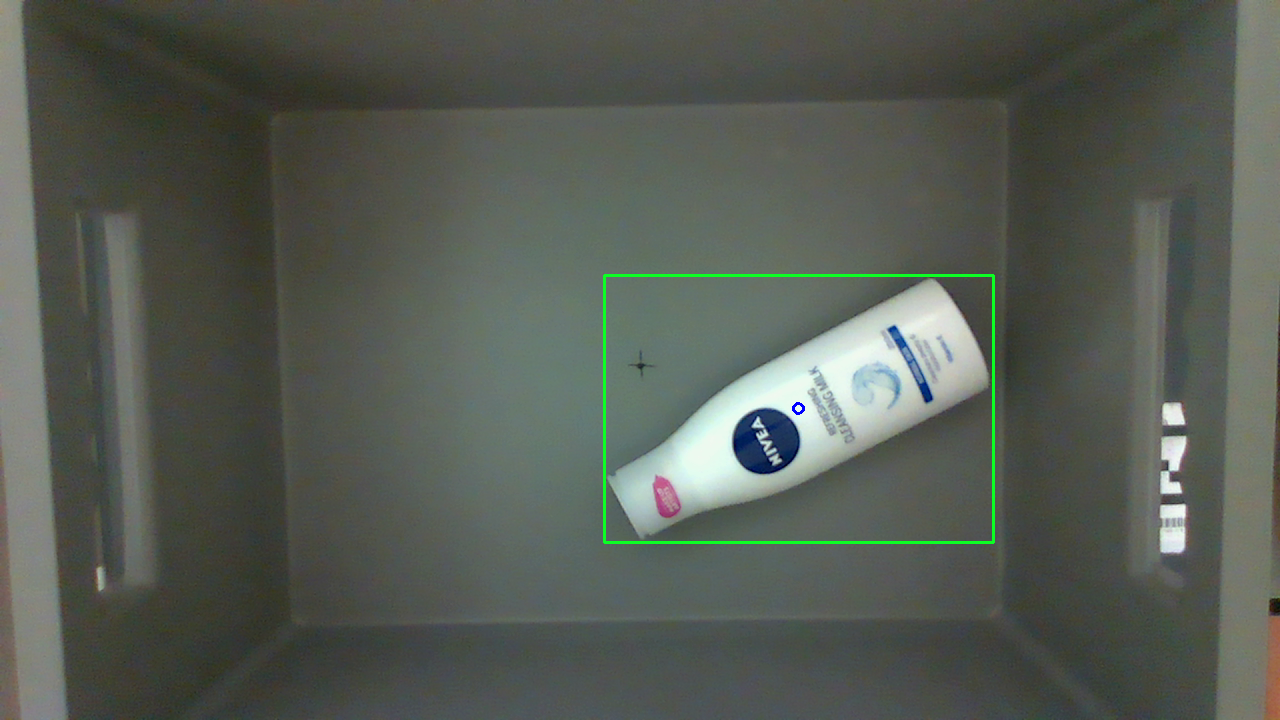
\includegraphics[width=0.495\textwidth]{graphics/results/niveacleansingmilk100_8.png}}
    \hfill
    \subfloat[Nivea Elastic]{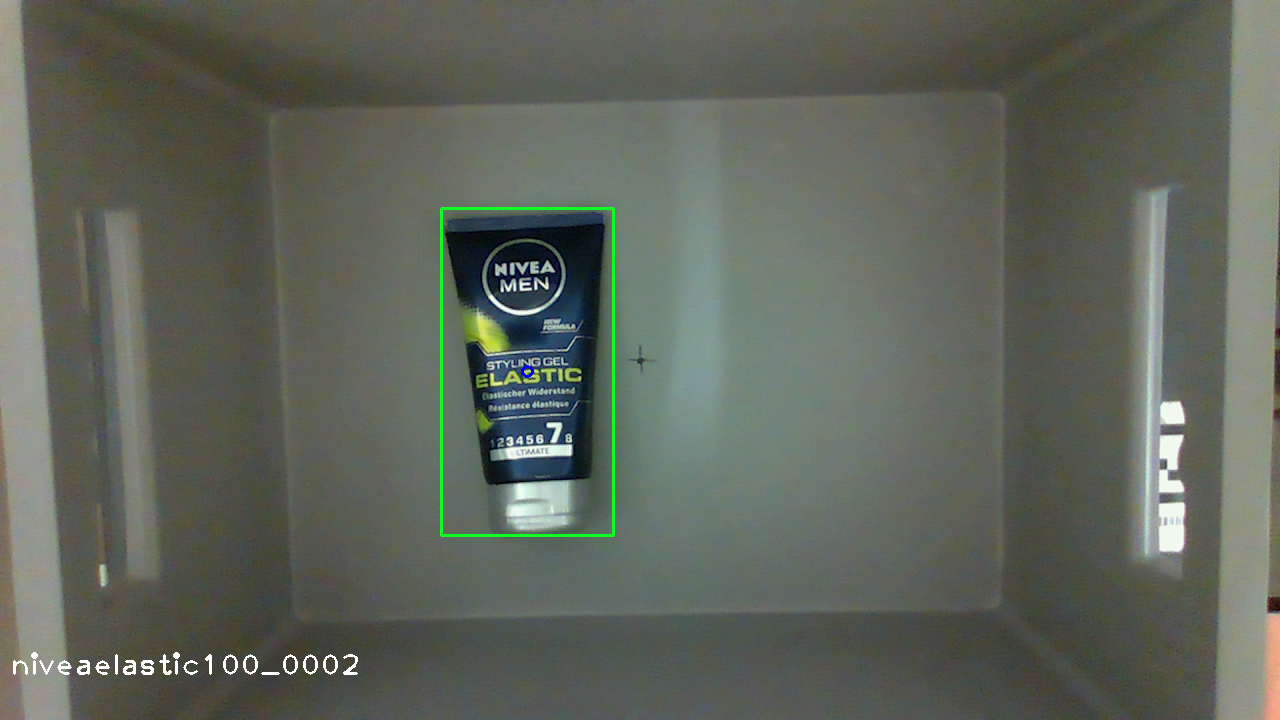
\includegraphics[width=0.495\textwidth]{graphics/results/niveaelastic100_0002box.png}}
    \hfill
    \subfloat[Nivea texture]{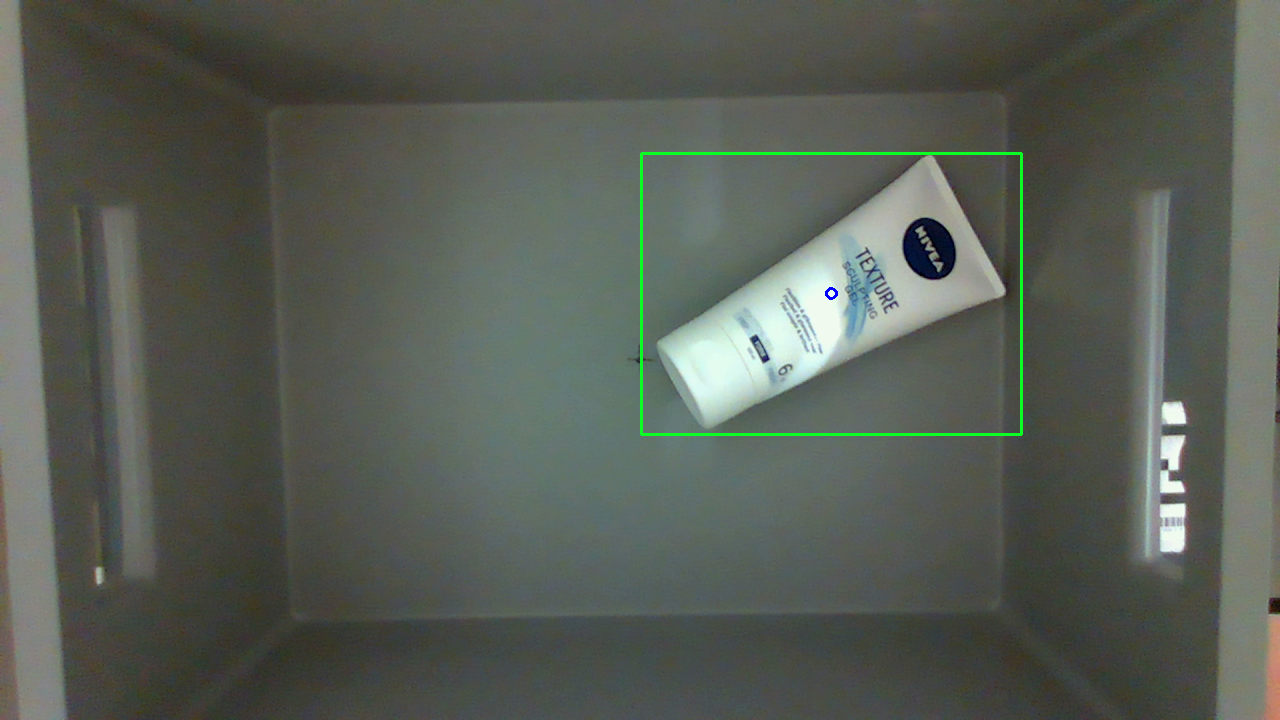
\includegraphics[width=0.495\textwidth]{graphics/results/niveatexture70_27.png}}
    \caption{The results from the difference.py, which shows the bounding box of four products}
    \label{figure: labelling}
\end{figure}


Since this method worked to created automatic labelled data, an test was made on the code how long would it take to label one image. Results from that test can been seen in \textit{Table \ref{tab:timediff}} and there it can be seen that it takes on average 0.85 second to label one image. 
\vspace{1cm}

\begin{table}[h]
\resizebox{\textwidth}{!}{%
\begin{tabular}{clccc}
\hline
\multicolumn{1}{l|}{\textit{Test \#}} &
  \textit{Item} &
  \multicolumn{1}{l}{\textit{Images}} &
  \multicolumn{1}{l}{\textit{Time {[}s{]}}} &
  \multicolumn{1}{l}{\textit{Time per image {[}s{]}}} \\ \hline
\multicolumn{1}{c|}{1} & \begin{tabular}[c]{@{}l@{}}Nivea\\ cleansing milk\end{tabular}    & 300 & 255.99 & 0.85 \\
\multicolumn{1}{c|}{2} & \begin{tabular}[c]{@{}l@{}}Nivea\\ cleansing milk\end{tabular}    & 102 & 92.68  & 0.91 \\
\multicolumn{1}{c|}{3} & \begin{tabular}[c]{@{}l@{}}Nivea \\ elastic\end{tabular}          & 72  & 56.31  & 0.78 \\
\multicolumn{1}{c|}{4} & \begin{tabular}[c]{@{}l@{}}Alberto \\ Balsam coconut\end{tabular} & 102 & 88.30  & 0.87 \\ \hline
\multicolumn{4}{r}{Average:}                                                                              & 0.85
\end{tabular}%
}
\caption{Measured time when using the difference.py}
\label{tab:timediff}
\end{table}

\clearpage
%%%%%%%%%%%%%%%%%%%%%%%%%%%%%%%%%%%%%%%%%%%%%%%%%%%%%%%%%%%%%%%%%%%%%
\section{Creating a new model for object detection}\label{reslabelled}
\begin{figure}[h]
    \centering
    % include first image
    \subfloat[Using YOLOv4]{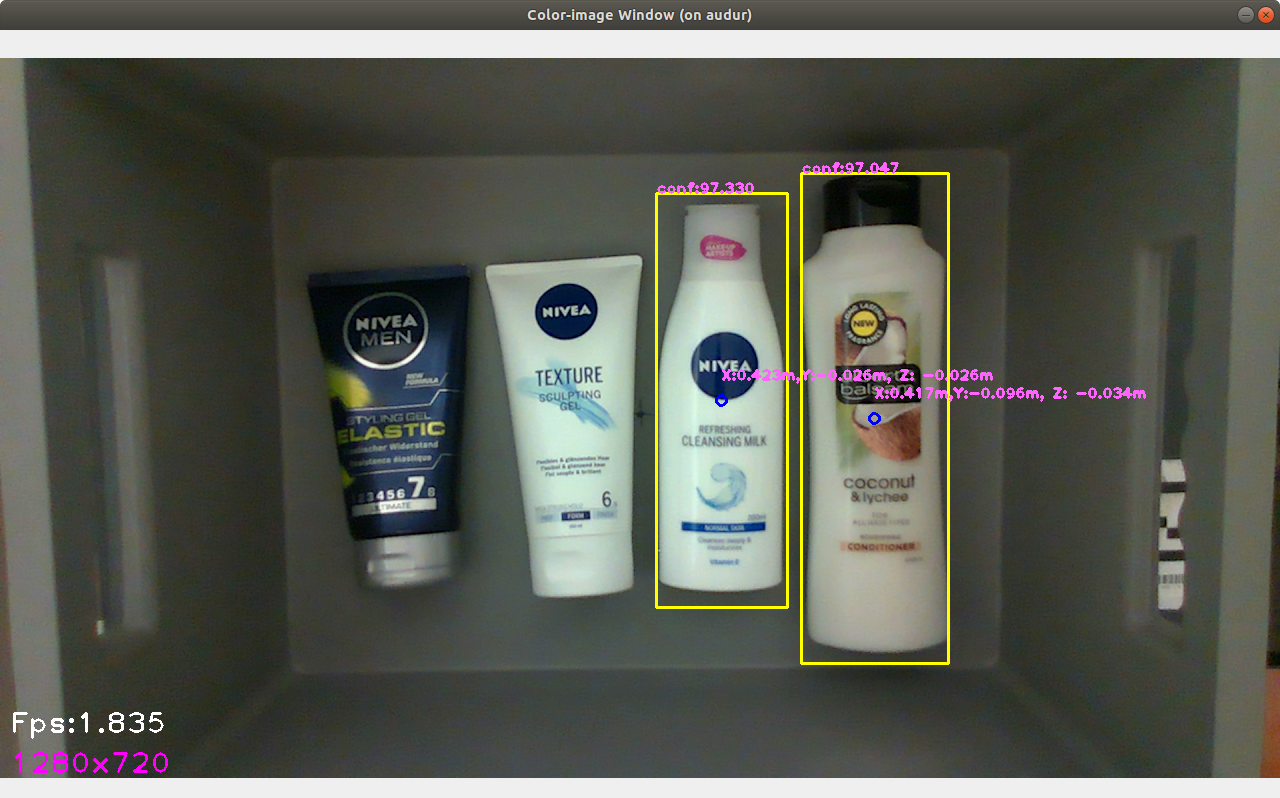
\includegraphics[width=0.495\textwidth]{graphics/results/beforetraining.png}}
    \hfill
    \subfloat[Using trained YOLOv4]{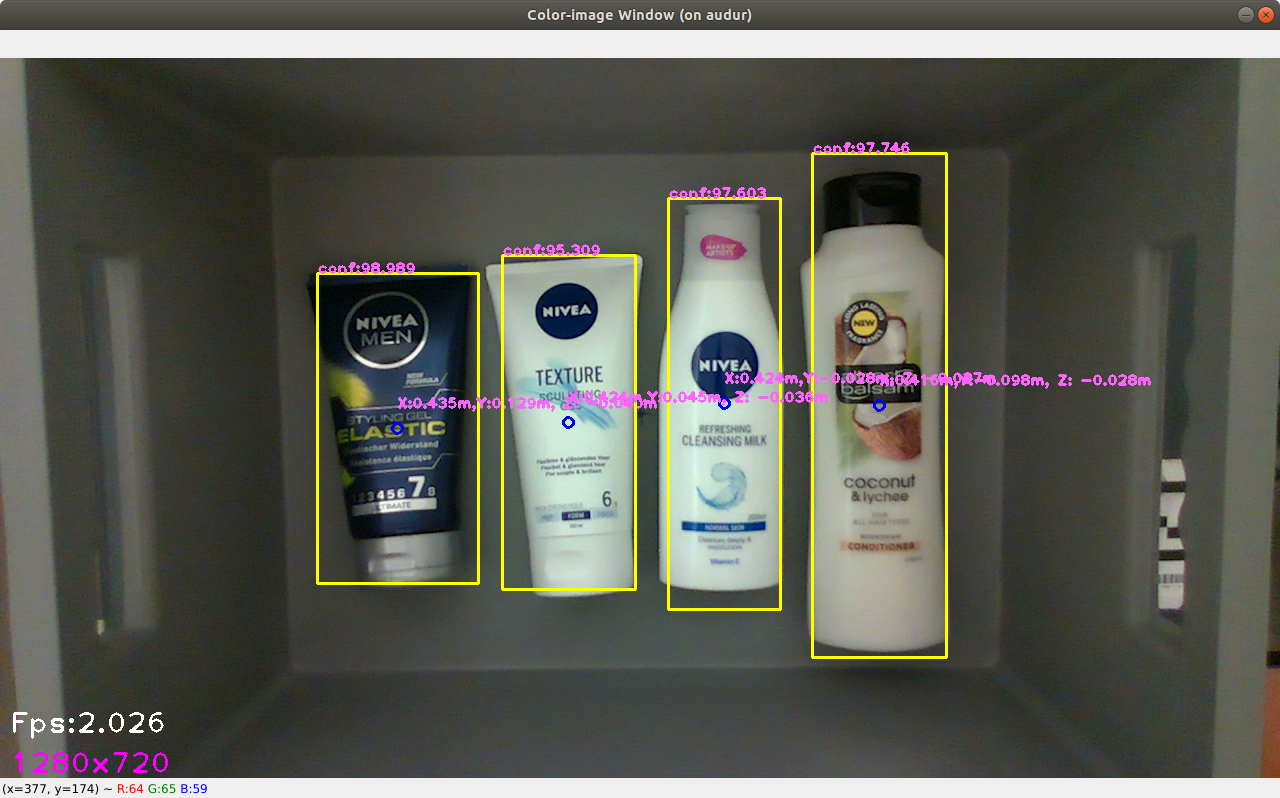
\includegraphics[width=0.495\textwidth]{graphics/results/aftertraining.png}}
    \hfill
    \subfloat[Using YOLOv4]{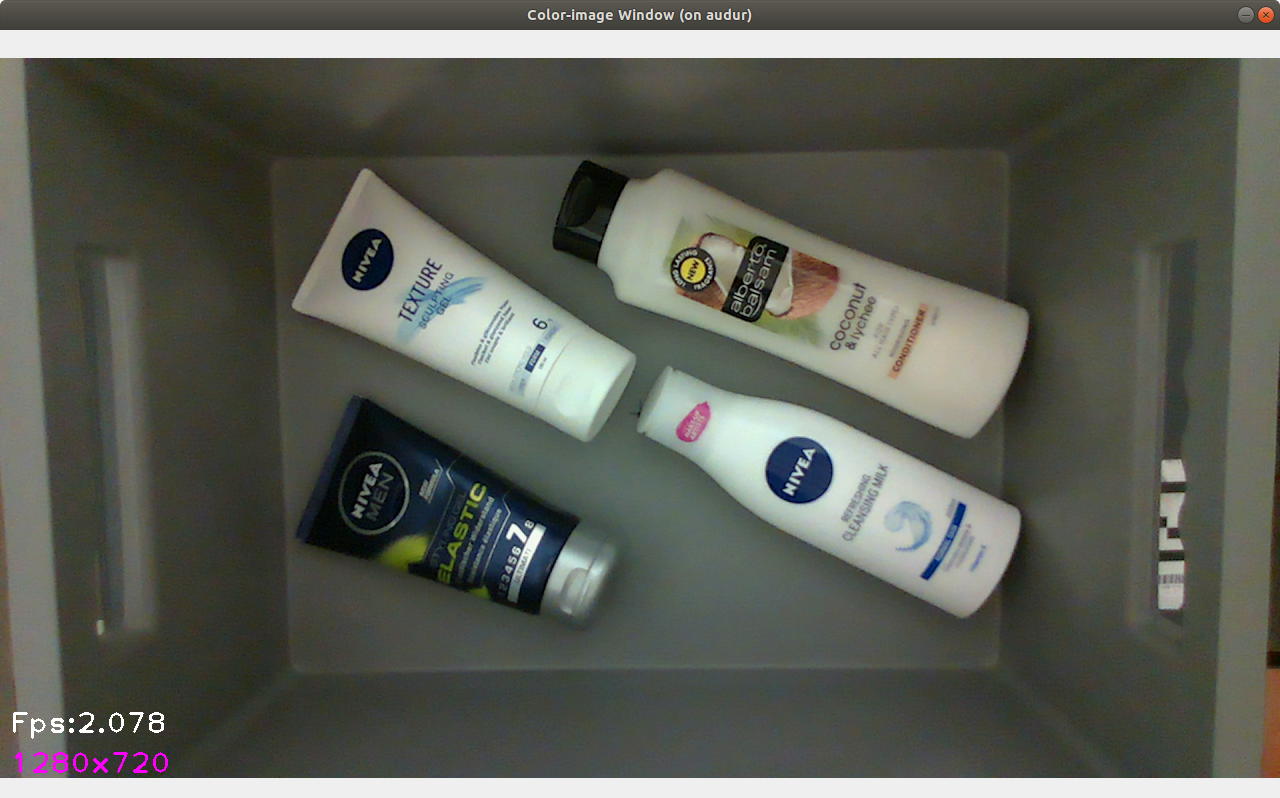
\includegraphics[width=0.495\textwidth]{graphics/results/beforetraining1.png}}
    \hfill
    \subfloat[Using trained YOLOv4]{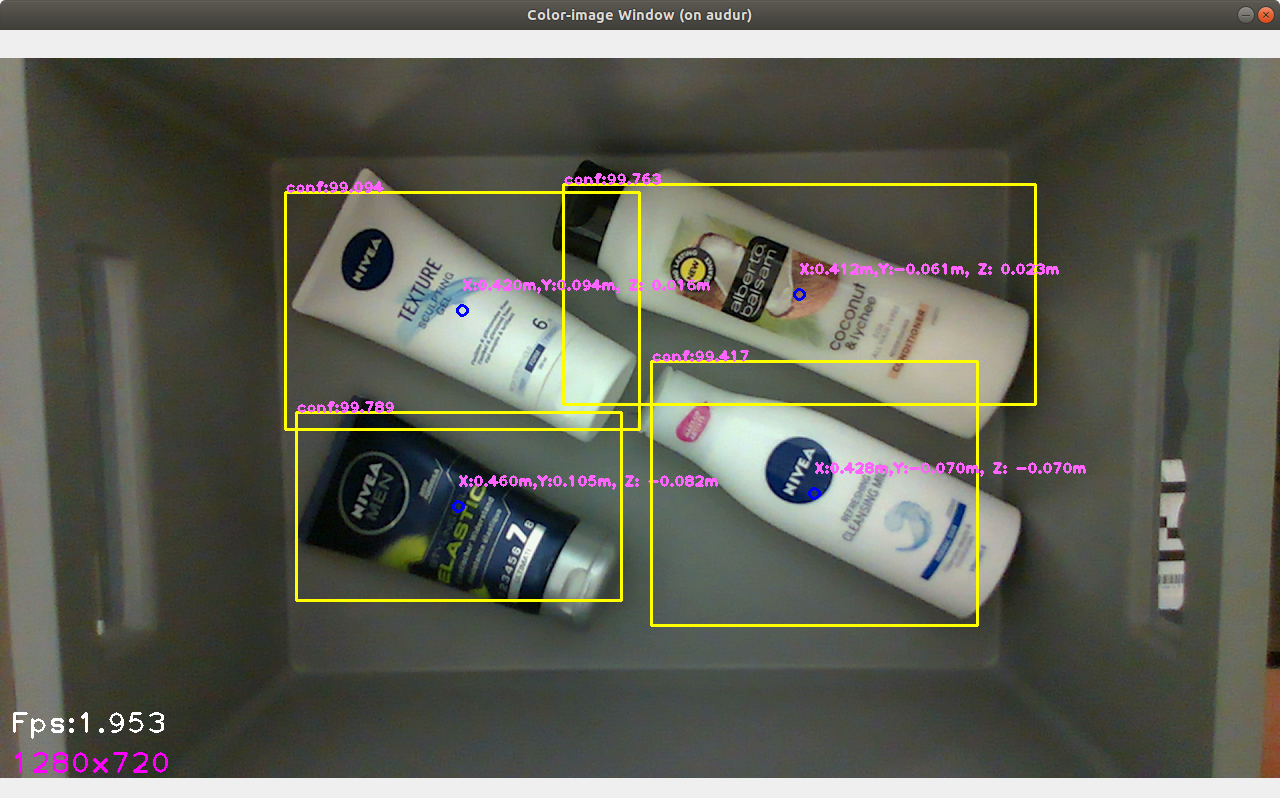
\includegraphics[width=0.495\textwidth]{graphics/results/aftertraining1.png}}
    \hfill
    \subfloat[Using YOLOv4]{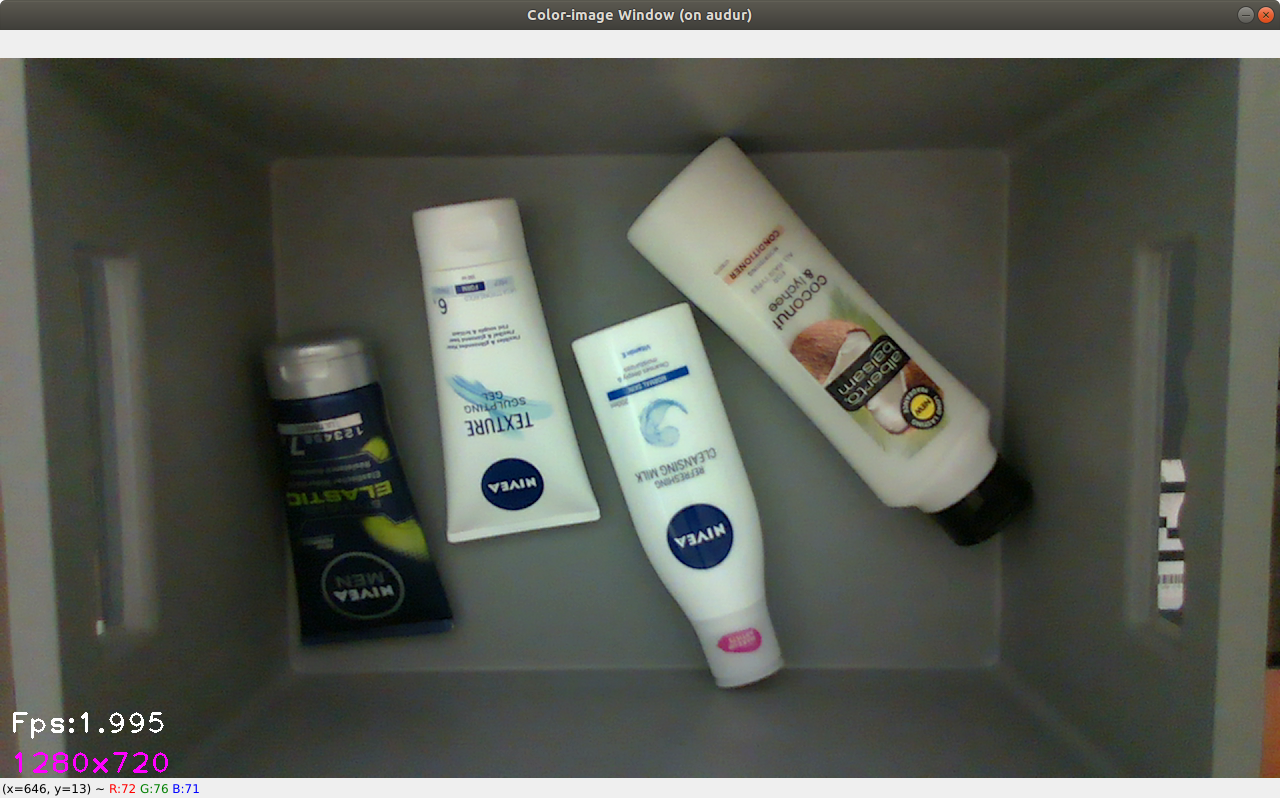
\includegraphics[width=0.495\textwidth]{graphics/results/beforetraining2.png}}
    \hfill
    \subfloat[Using trained YOLOv4]{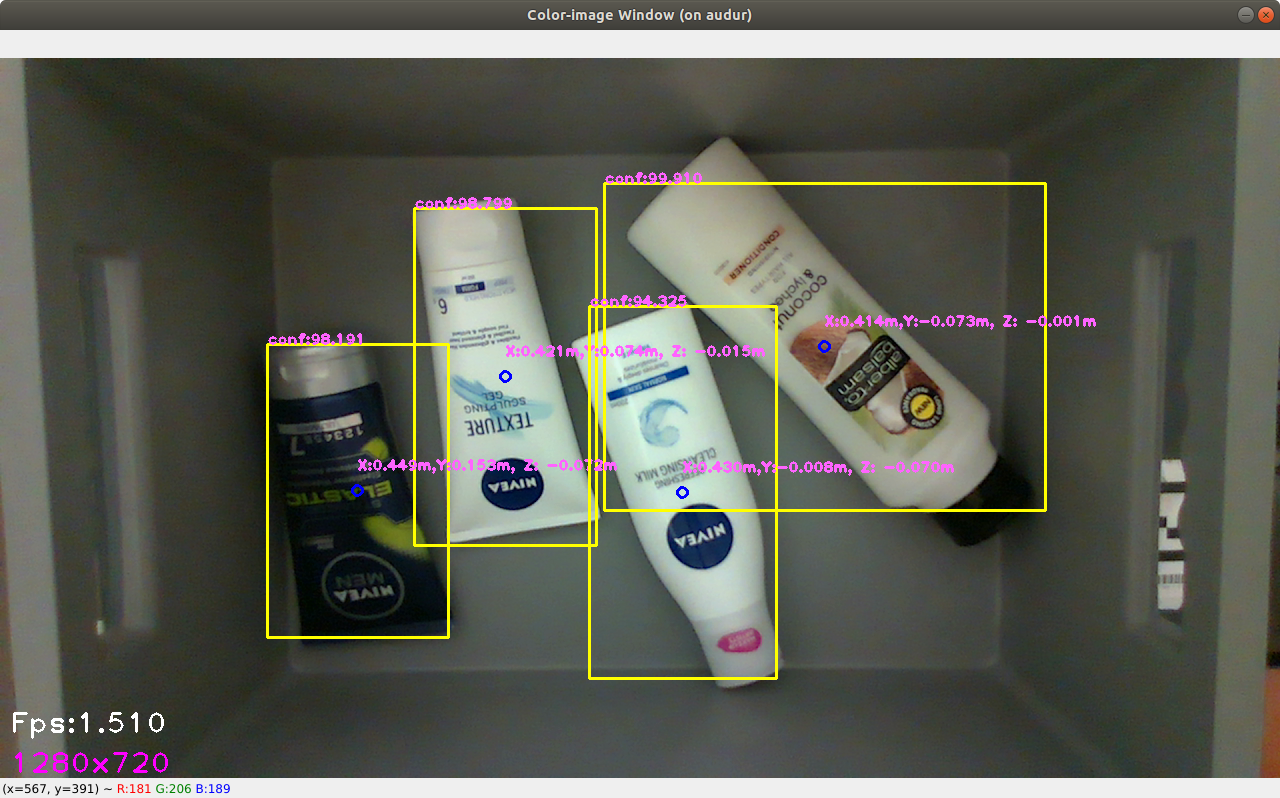
\includegraphics[width=0.495\textwidth]{graphics/results/aftertraining2.png}}
    \caption{Using YOLOv4 and the trained YOLOv4 model, trained on images from the robot}
    \label{figure: beforeaftertraining}
\end{figure}

\clearpage
\section{Results from the first neural network}
\begin{figure}[h]
    \centering
    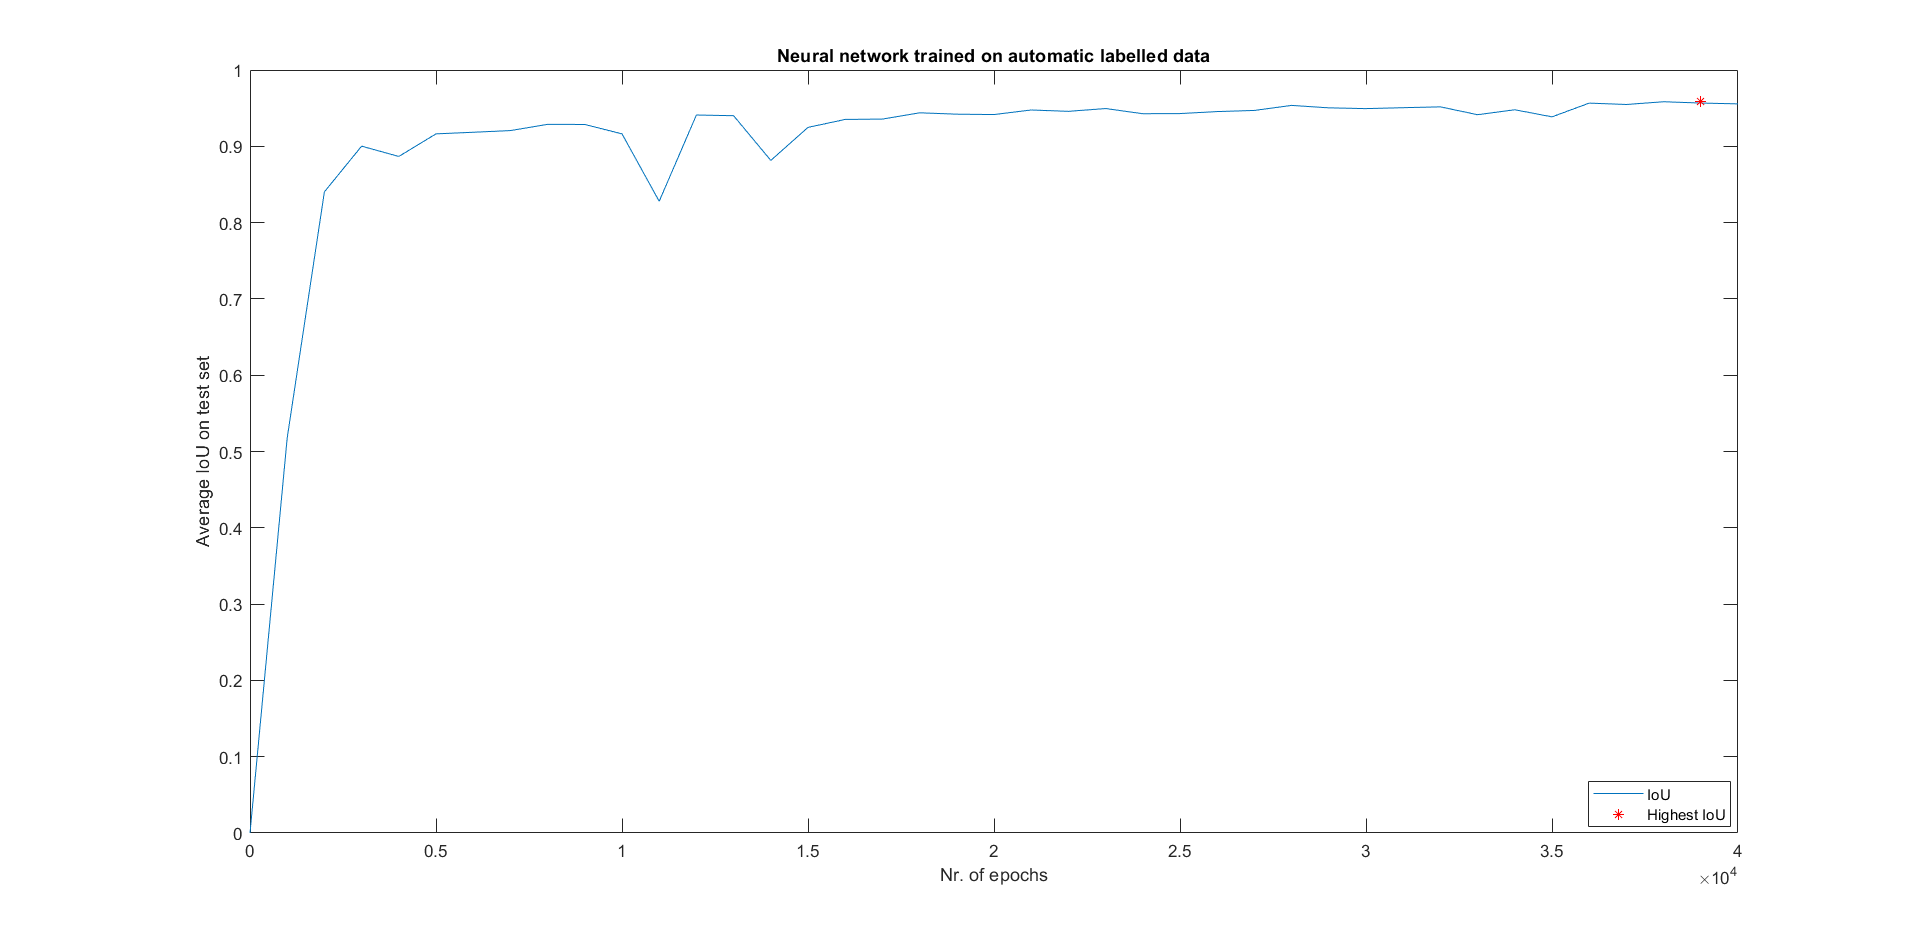
\includegraphics[width=1\textwidth]{graphics/results/neuralnetworkauto.png}
    \caption{IoU every 1000 epochs}
    \label{fig:neuralnetwork}
\end{figure}

\subsection{On trained items}

\begin{figure}[h]
    \centering
    % include first image
    \subfloat[Alberto Balsam]{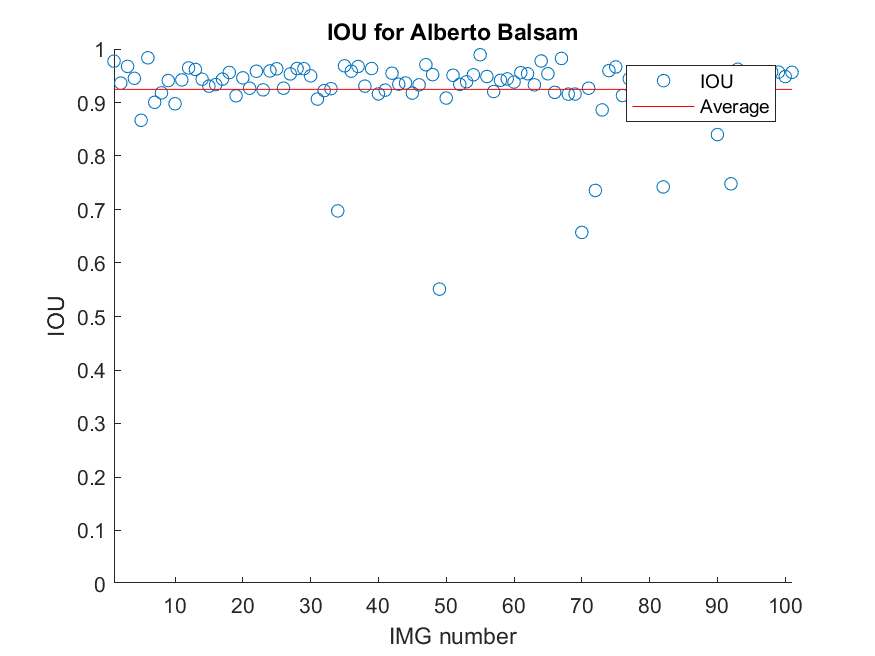
\includegraphics[width=0.495\textwidth]{graphics/albertobalsamIOU.png}}
    \hfill
    \subfloat[Nivea Cleansing Milk]{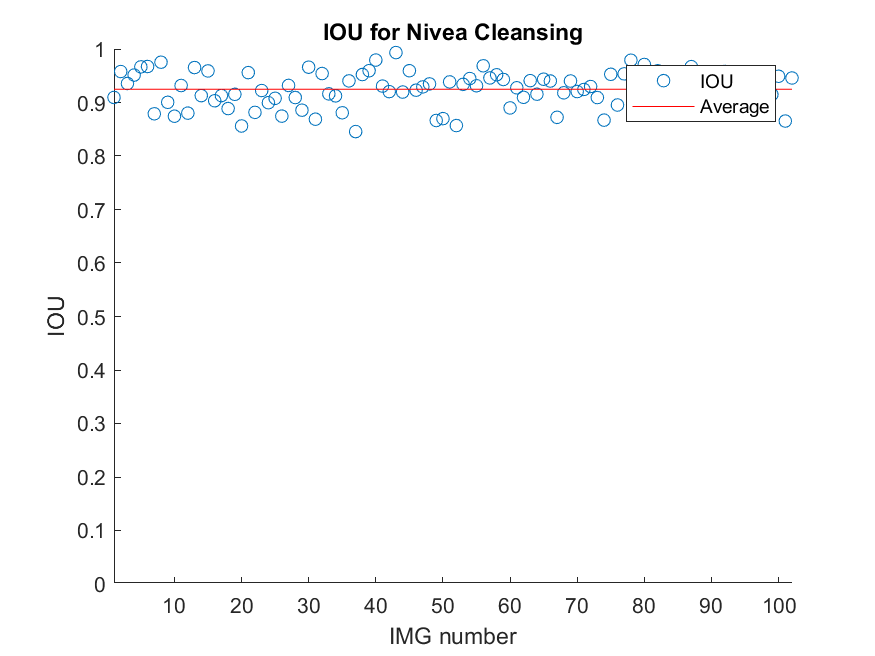
\includegraphics[width=0.495\textwidth]{graphics/niveacleansingIOU.png}}
    \hfill
    \subfloat[Nivea Elastic]{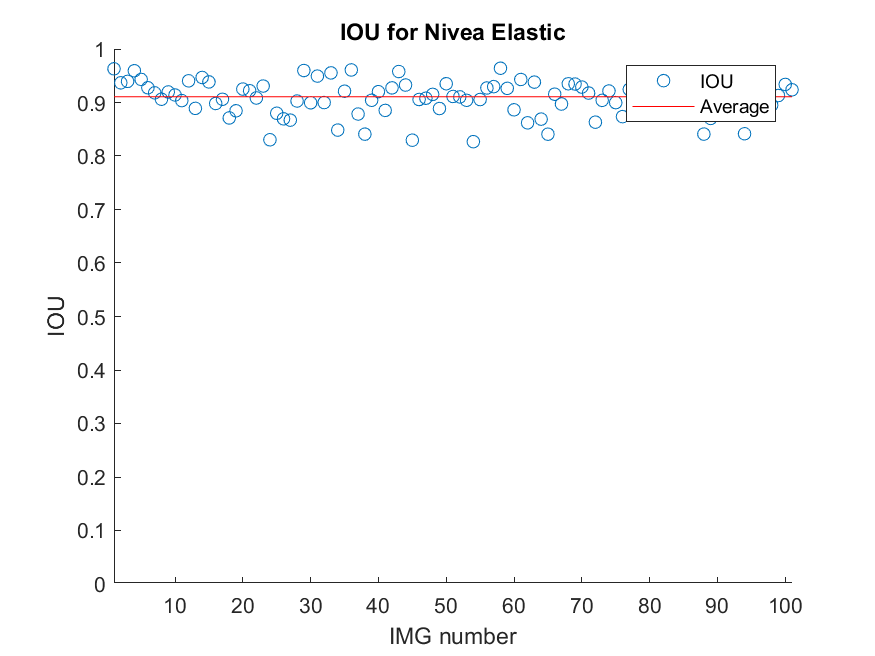
\includegraphics[width=0.495\textwidth]{graphics/niveaelasticIOU.png}}
    \hfill
    \subfloat[Nivea Texture]{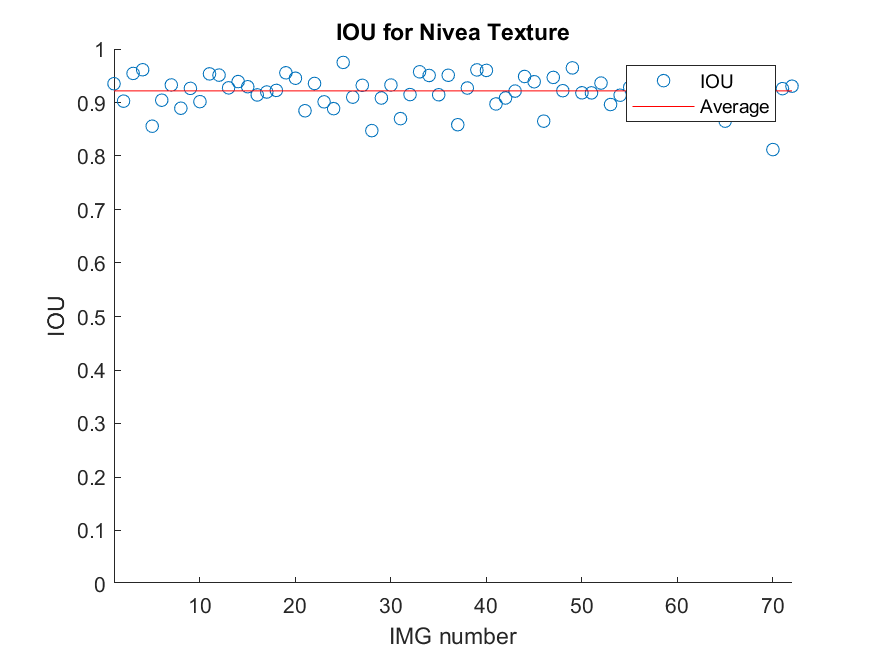
\includegraphics[width=0.495\textwidth]{graphics/niveatextureIOU.png}}
    \caption{Scatter plot for IoU on known products}
    \label{figure: knownproducts}
\end{figure}


\begin{table}[h]
\resizebox{\textwidth}{!}{%
\begin{tabular}{l|cccccccc}
\hline
\textit{Item} &
  \textit{Products} &
  \textit{Detections} &
  \textit{True Positive} &
  \textit{False Positive} &
  \textit{Avg-IoU} &
  \textit{Avg-Precision} &
  \textit{Avg-Recall} &
  \textit{Avg-F1} \\ \hline
Alberto Balsam & 101 & 101 & 101 & 0 & 0.9244 & 1 & 1 & 1 \\
Nivea C. Milk & 102 & 102 & 102 & 0 & 0.9248 & 1 & 1 & 1 \\
Nivea Elastic & 101 & 101 & 101 & 0 & 0.9107 & 1 & 1 & 1 \\
Nivea Texture & 72  & 72  & 72  & 0 & 0.9217 & 1 & 1 & 1 \\ \hline
\end{tabular}%
}
\caption{The results when tested on trained data}
\label{tab:ready}
\end{table}


\begin{figure}[h]
    \centering
    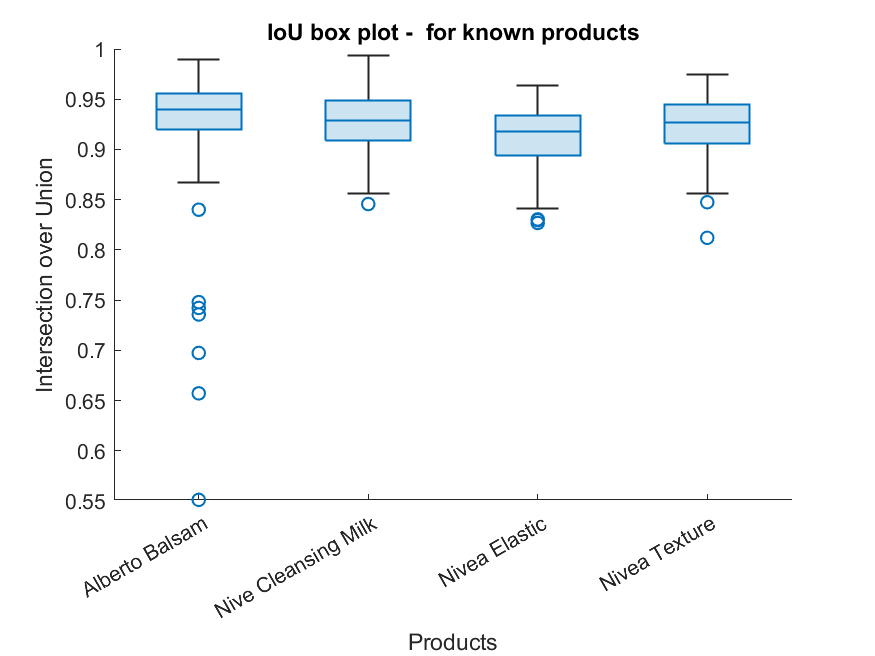
\includegraphics[width=0.9\textwidth]{graphics/results/boxplotForKnownProducts.png}
    \caption{Box plot for known products}
    \label{fig:boxknownproducts}
\end{figure}

\clearpage
\subsection{On unknown Beiersdorf products}
\begin{figure}[h]
    \centering
    % include first image
    \subfloat[Item 11]{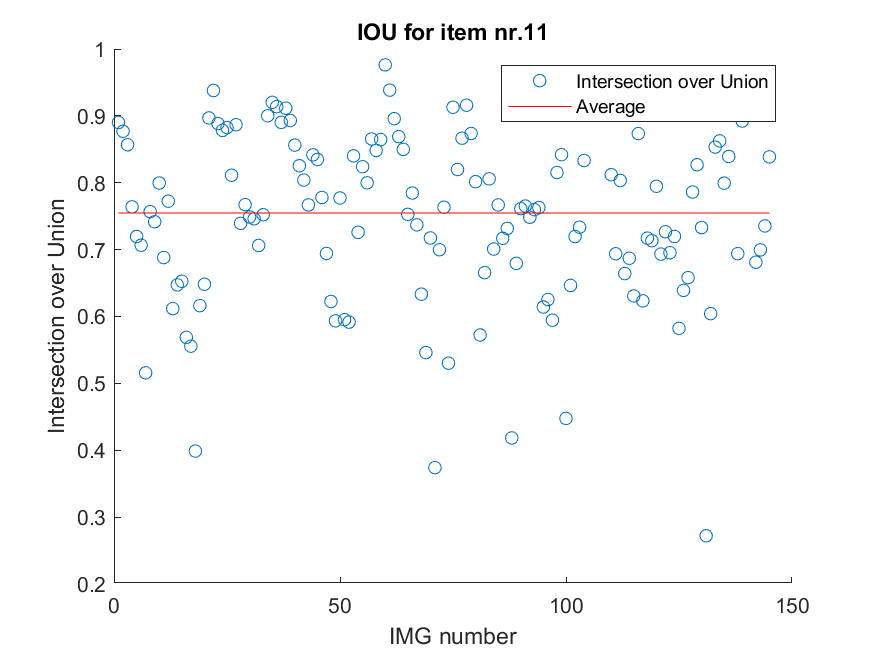
\includegraphics[width=0.495\textwidth]{graphics/results/item11.png}}
    \hfill
    \subfloat[Item 12]{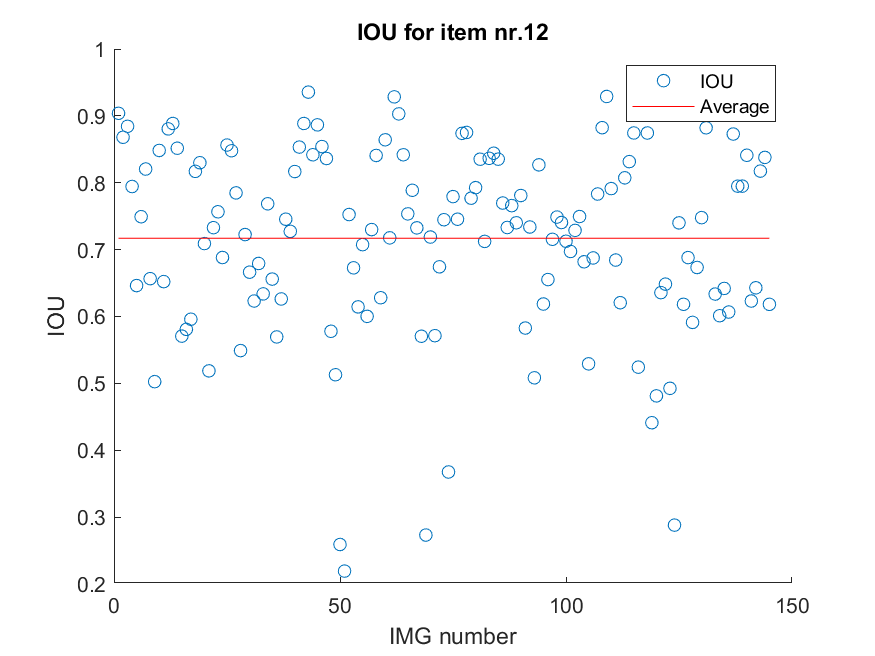
\includegraphics[width=0.495\textwidth]{graphics/results/item12.png}}
    \hfill
    \subfloat[Item 5]{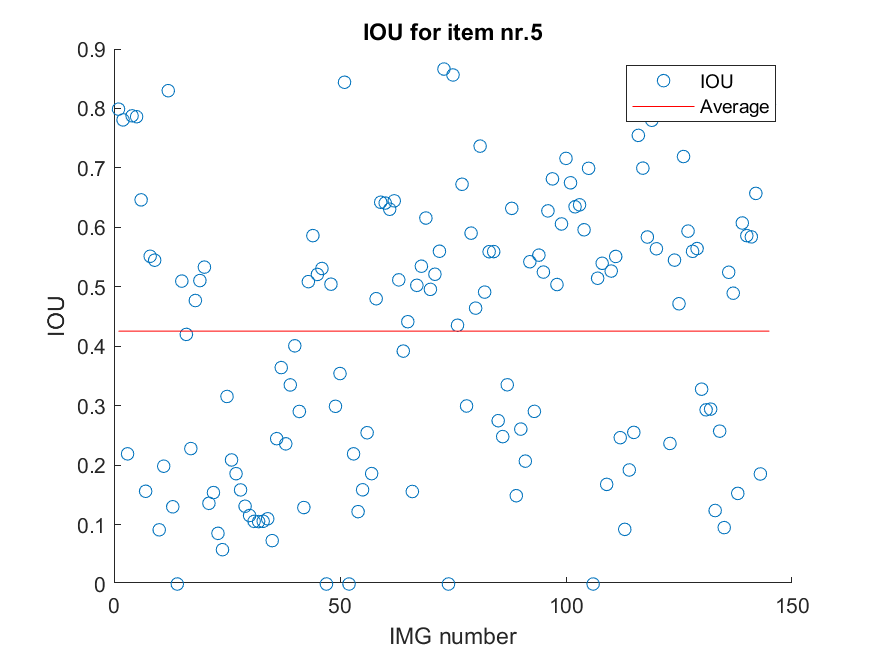
\includegraphics[width=0.495\textwidth]{graphics/results/item5.png}}
    \hfill
    \subfloat[Item 6]{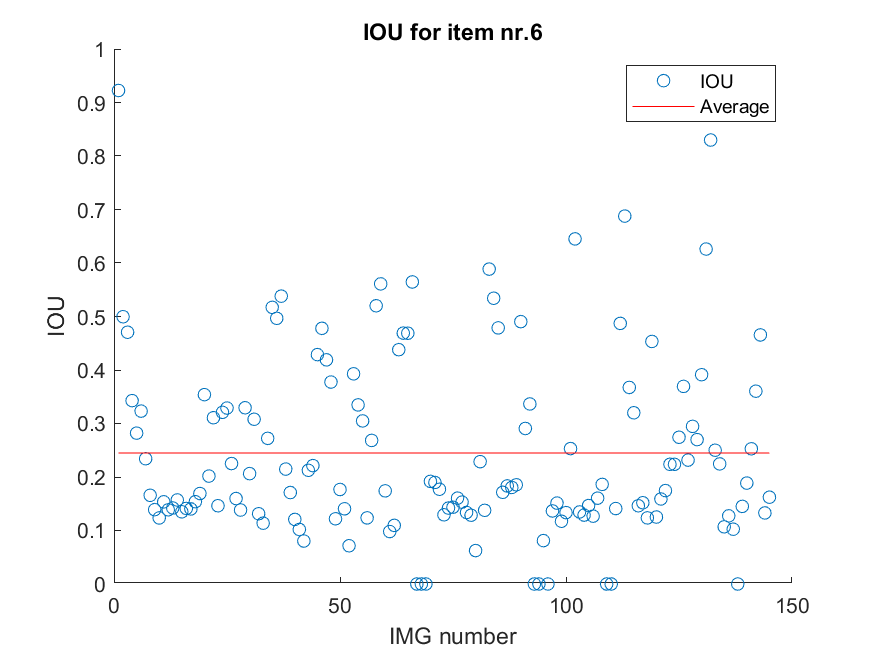
\includegraphics[width=0.495\textwidth]{graphics/results/item6.png}}
    
    \label{figure: unknownproducts}
    \caption{Scatter plot for IoU on unknown products}
\end{figure}

\begin{table}[h]
\resizebox{\textwidth}{!}{%
\begin{tabular}{c|cccccccc}
\hline
\textit{Item} &
  \textit{Products} &
  \textit{Detections} &
  \textit{True Positive} &
  \textit{False Positive} &
  \textit{Avg-IoU} &
  \textit{Avg-Precision} &
  \textit{Avg-Recall} &
  \textit{Avg-F1} \\ \hline
1  & 684  & 332 & 300 & 29  & 0.648  & 0.8299 & 0.5032 & 0.595  \\
2  & 1029 & 392 & 330 & 55  & 0.579  & 0.7327 & 0.3862 & 0.471  \\
3  & 667  & 368 & 337 & 29  & 0.6734 & 0.8523 & 0.569  & 0.6542 \\
4  & 683  & 350 & 325 & 24  & 0.7058 & 0.8891 & 0.5426 & 0.6394 \\
5  & 892  & 317 & 202 & 110 & 0.4253 & 0.5205 & 0.2418 & 0.3194 \\
6  & 918  & 195 & 57  & 129 & 0.2449 & 0.1833 & 0.0682 & 0.0956 \\
7  & 851  & 405 & 326 & 78  & 0.5757 & 0.7314 & 0.3907 & 0.4956 \\
8  & 788  & 292 & 264 & 26  & 0.664  & 0.8615 & 0.3707 & 0.4895 \\
9  & 887  & 333 & 270 & 60  & 0.536  & 0.7218 & 0.3308 & 0.4349 \\
10 & 665  & 344 & 293 & 51  & 0.626  & 0.7736 & 0.4761 & 0.5667 \\
11 & 627  & 385 & 361 & 23  & 0.7245 & 0.8994 & 0.623  & 0.7106 \\
12 & 574  & 417 & 394 & 23  & 0.7171 & 0.9268 & 0.7376 & 0.7971 \\
13 & 618  & 307 & 291 & 14  & 0.694  & 0.9149 & 0.5309 & 0.6403 \\
14 & 1031 & 245 & 180 & 52  & 0.5178 & 0.6299 & 0.2211 & 0.3012 \\
15 & 616  & 302 & 273 & 23  & 0.6897 & 0.8368 & 0.4918 & 0.5858 \\ 
\hline
\end{tabular}%
}
\caption{The results when tested on unknown data}
\label{tab:test1unknown}
\end{table}
\begin{figure}[h]
    \centering
    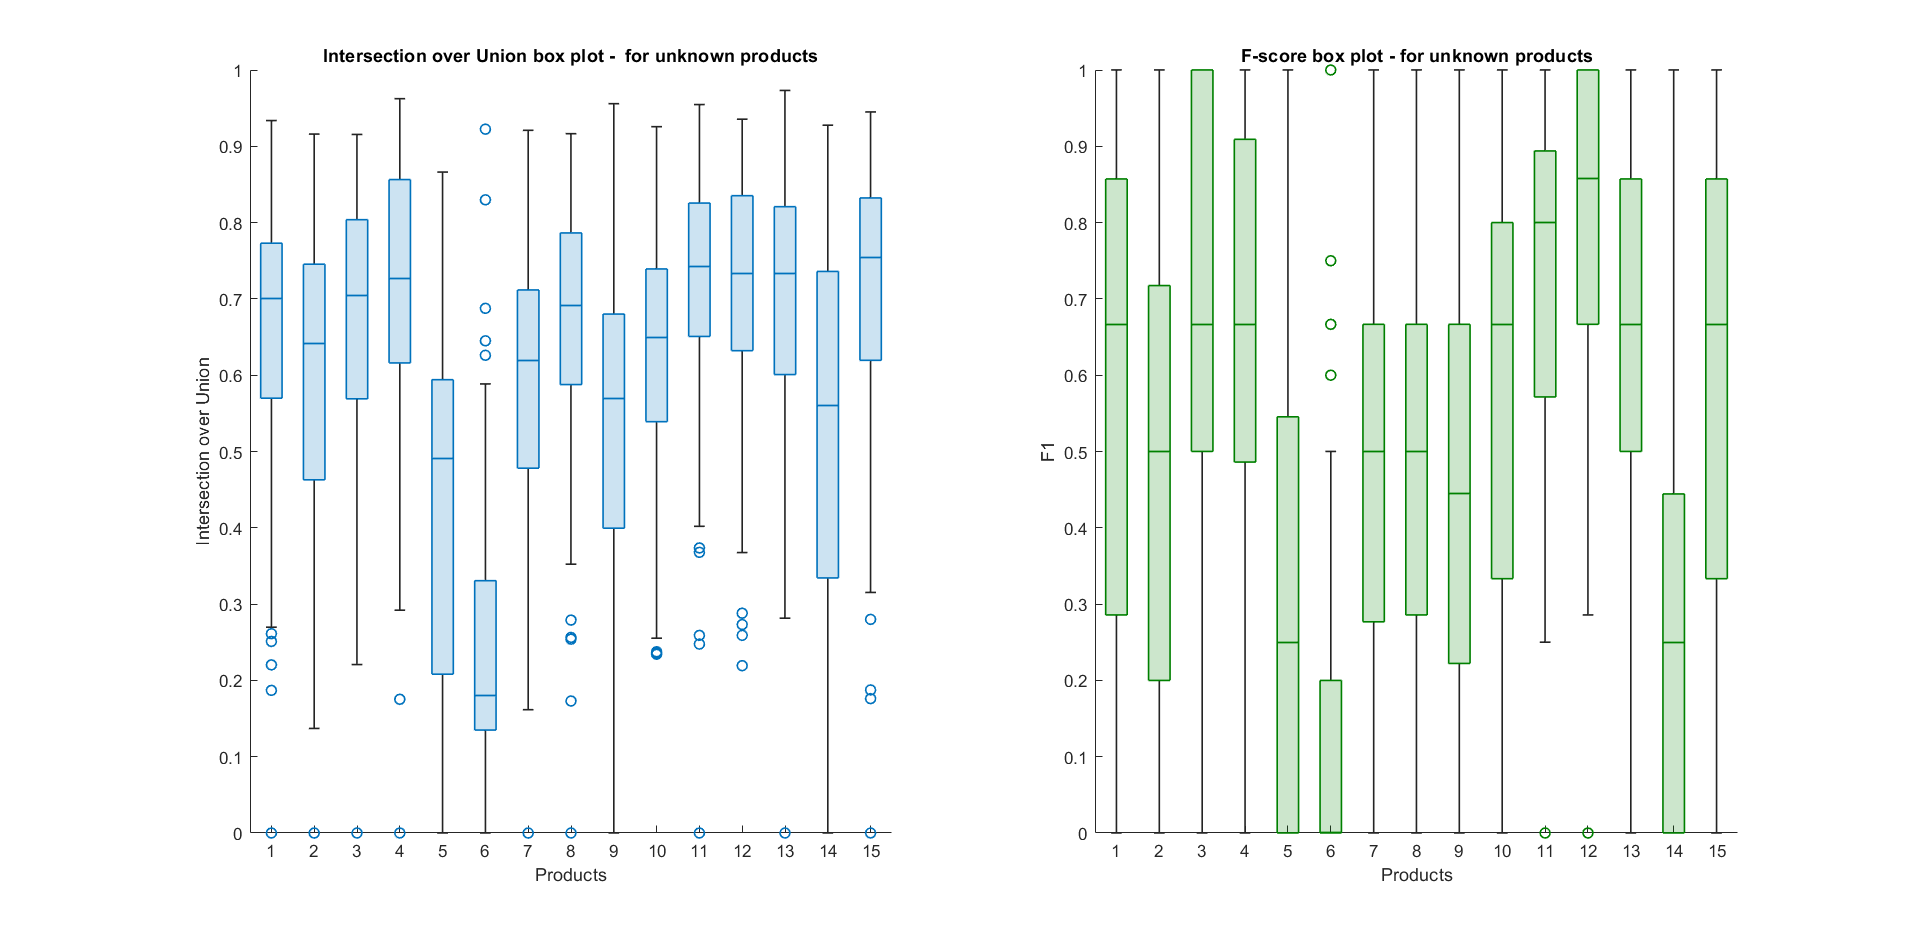
\includegraphics[width=1\textwidth, trim={5cm 0 5cm 0},clip]{graphics/results/boxplotForProducts.png}
    \caption{Box plot for unknown products, Intersection over Union on the left and F-score on the right}
    \label{fig:boxunknownproducts}
\end{figure}

\begin{figure}[h]
    \centering
    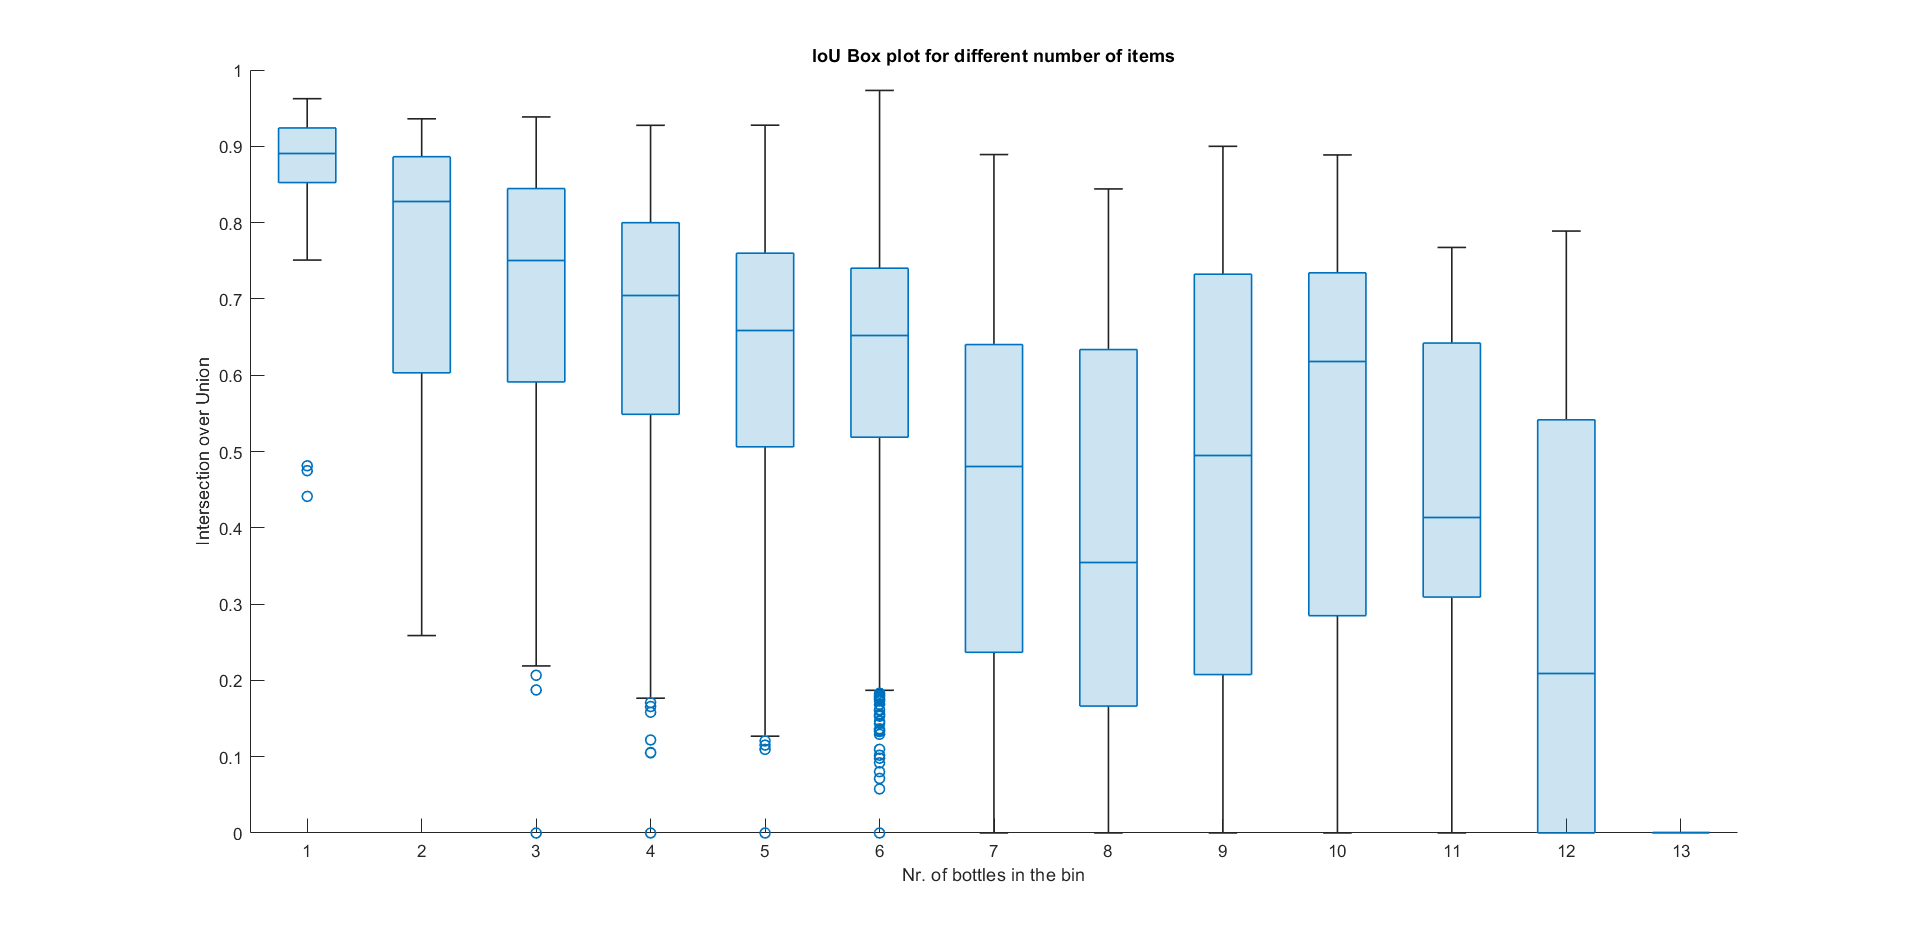
\includegraphics[width=1\textwidth]{graphics/results/boxplotBottles.png}
    \caption{IoU box plot for different number of items}
    \label{fig:bottles}
\end{figure}